\chapter{Pengenalan Arsitektur Perangkat Lunak dan Arsitektur Client-Server}


\section{Pendahuluan}

Arsitektur perangkat lunak merupakan elemen fundamental dalam pengembangan sistem modern. Sebagai kerangka kerja yang mendefinisikan struktur, komponen, dan hubungan antar elemen dalam suatu sistem perangkat lunak, arsitektur memiliki peran yang sangat penting dalam menentukan skalabilitas, keandalan, keamanan, dan kemudahan pemeliharaan suatu aplikasi. Dengan meningkatnya kompleksitas sistem perangkat lunak, pemilihan arsitektur yang tepat menjadi faktor kunci dalam keberhasilan implementasi dan evolusi sistem.

Bab ini membahas berbagai aspek arsitektur perangkat lunak, dimulai dengan definisi dan konsep dasar yang menjadi landasan dalam perancangannya. Prinsip-prinsip utama seperti modularitas, skalabilitas, kinerja, keamanan, serta maintainability dijelaskan secara mendalam untuk memberikan pemahaman mengenai faktor-faktor yang harus dipertimbangkan dalam membangun sistem yang efektif. Teknik-teknik yang digunakan dalam mendukung implementasi prinsip-prinsip tersebut juga diuraikan, termasuk penggunaan arsitektur berlapis, desain berbasis mikroservis, serta pendekatan event-driven yang semakin umum digunakan dalam sistem modern.

Untuk memberikan pemahaman yang lebih kontekstual, beberapa studi kasus disajikan guna menunjukkan bagaimana keputusan arsitektural dapat berkontribusi terhadap keberhasilan atau kegagalan suatu sistem. Kasus transformasi arsitektur Netflix dari sistem monolitik ke mikroservis menggambarkan bagaimana arsitektur yang fleksibel dapat meningkatkan skalabilitas dan kinerja layanan. Sebaliknya, kegagalan Healthcare.gov menyoroti dampak dari desain arsitektur yang buruk terhadap stabilitas dan pengalaman pengguna. Selain itu, penerapan arsitektur event-driven dalam industri perbankan menunjukkan bagaimana pemrosesan transaksi real-time dapat dioptimalkan melalui pendekatan yang tepat.

Sebagai bagian dari pembahasan yang lebih teknis, bab ini juga mengeksplorasi arsitektur Client-Server, yang merupakan salah satu model komunikasi paling umum dalam sistem perangkat lunak. Latar belakang, struktur dasar, serta kelebihan dan kekurangan arsitektur Client-Server dianalisis untuk memberikan gambaran mengenai bagaimana model ini diterapkan dalam berbagai skenario. Studi kasus implementasi arsitektur Client-Server dalam lingkungan nyata juga disertakan untuk memperlihatkan bagaimana konsep ini dapat diadaptasi sesuai dengan kebutuhan bisnis dan teknis.

Melalui pembahasan ini, diharapkan pembaca dapat memahami pentingnya arsitektur perangkat lunak dalam membangun sistem yang andal, scalable, dan mudah dipelihara. Dengan memahami prinsip-prinsip dasar, teknik implementasi, serta studi kasus nyata, pembaca dapat menerapkan konsep-konsep yang telah dipelajari dalam pengembangan sistem perangkat lunak yang lebih efektif dan efisien.

Berikut adalah garis besar topik-topik yang dibahas dalam setiap bab:
\begin{enumerate}
\item Introduction to Software Architecture and Client-Server Architecture
\item Containers
\item Layered Architecture
\item Model-View-* (MV*) Architecture
\item Hexagonal Architecture
\item Microkernel Architecture
\item Peer-to-Peer (P2P) Architecture

\item Space-Based Architecture (SBA)
\item Pipeline / Pipe-and-Filter Architecture
\item Event-Driven Architecture (EDA)
\item Microservices Architecture
\item Orchestration-driven Service-Oriented Architecture (ODSOA)
\item Service-based (Serverless) Architecture
\item DevOps
\end{enumerate}


\section{Deskripsi Outcome-Based Education (OBE)}

Pendekatan Outcome-Based Education (OBE) dalam materi ini dirancang untuk memastikan bahwa mahasiswa memahami dan dapat menerapkan berbagai pola arsitektur dalam pengembangan perangkat lunak. Setiap pertemuan memiliki target formatif yang terukur (\textit{measurable outcome}) guna memastikan pemahaman yang progresif sebelum mencapai capaian sumatif di akhir.

\subsection{Capaian Formatif Per Pertemuan}

\begin{enumerate}

\item \textbf{Introduction to Software Architecture and Client-Server Architecture}  
\textbf{Target Formatif:} Mahasiswa memahami konsep dasar arsitektur perangkat lunak dan model Client-Server.  \\
\textbf{Measurable Outcomes:}
\begin{itemize}
\item Menjelaskan konsep dasar arsitektur perangkat lunak, termasuk prinsip modularitas dan skalabilitas.
\item Memahami kelebihan (\textit{scalability, modularity, maintainability}) dan kekurangan (\textit{overhead, latency, complexity}) dari arsitektur Client-Server.
\item Menggambarkan model komunikasi Client-Server dan membandingkannya dengan arsitektur monolitik dalam aspek efisiensi dan pemrosesan data.
\item Mengembangkan implementasi sederhana dari komunikasi Client-Server dan mengevaluasi latensi serta keamanan data dalam komunikasi terdistribusi.
\end{itemize}

\item \textbf{Containers}  
\textbf{Target Formatif:} Mahasiswa memahami konsep containerization dan bagaimana Docker serta OCI menjadi fondasi bagi Kubernetes dan DevOps.  \\
\textbf{Measurable Outcomes:}
\begin{itemize}
\item Menjelaskan konsep containerization dan perbedaannya dengan virtualisasi tradisional dalam hal efisiensi sumber daya dan isolasi lingkungan.
\item Memahami kelebihan (\textit{portability, scalability, rapid deployment}) dan kekurangan (\textit{security risks, persistent storage issues}) dari containerization.
\item Menginstal dan mengkonfigurasi Docker serta menjalankan aplikasi dalam kontainer untuk memahami dampak performa terhadap sistem.
\item Mengembangkan aplikasi sederhana yang berjalan dalam kontainer Docker serta menguji skalabilitas dan efisiensinya.
\end{itemize}

\item \textbf{Layered Architecture}  
\textbf{Target Formatif:} Mahasiswa memahami dan mampu menerapkan struktur berlapis dalam desain perangkat lunak.  \\
\textbf{Measurable Outcomes:}
\begin{itemize}
\item Menjelaskan prinsip dasar arsitektur berlapis dan bagaimana pemisahan logika meningkatkan modularitas serta fleksibilitas pengembangan.
\item Memahami kelebihan (\textit{code reusability, separation of concerns}) dan kekurangan (\textit{performance overhead, complexity in debugging}) dari arsitektur berlapis.
\item Mendesain aplikasi sederhana menggunakan arsitektur berlapis dan mengevaluasi dampaknya terhadap pemeliharaan kode.
\item Mengimplementasikan aplikasi dengan pemisahan lapisan presentasi, bisnis, dan data untuk mengidentifikasi bottleneck kinerja.
\end{itemize}

\item \textbf{Model-View-* (MV*) Architecture}  
\textbf{Target Formatif:} Mahasiswa memahami pola desain MVC, MVVM, dan variasinya dalam pengembangan perangkat lunak.  \\
\textbf{Measurable Outcomes:}
\begin{itemize}
\item Menjelaskan perbedaan antara berbagai pola Model-View-* dan bagaimana masing-masing pola berdampak pada pengelolaan state aplikasi.
\item Memahami kelebihan (\textit{better UI management, separation of concerns}) dan kekurangan (\textit{complexity, overhead in event handling}) dari masing-masing pola Model-View-*.
\item Mendesain sistem antarmuka pengguna berdasarkan pola Model-View-* serta menganalisis trade-off dalam hal fleksibilitas dan kompleksitas implementasi.
\item Mengembangkan aplikasi sederhana menggunakan pola MVC atau MVVM dan mengevaluasi keterbatasan masing-masing pendekatan dalam pemrosesan data dan event.
\end{itemize}

\item \textbf{Hexagonal Architecture}  
\textbf{Target Formatif:} Mahasiswa memahami konsep modularitas dan pengujian dalam arsitektur Heksagonal.  \\
\textbf{Measurable Outcomes:}
\begin{itemize}
\item Menjelaskan konsep Ports and Adapters dalam arsitektur Heksagonal serta bagaimana pendekatan ini meningkatkan modularitas dan testability.
\item Memahami kelebihan (\textit{maintainability, decoupling, testability}) dan kekurangan (\textit{increased complexity, additional learning curve}) dari arsitektur Hexagonal.
\item Mendesain sistem modular menggunakan pendekatan Hexagonal dan mengevaluasi tantangan dalam implementasinya.
\item Mengembangkan aplikasi sederhana dengan pendekatan Hexagonal Architecture dan membandingkan fleksibilitasnya dengan arsitektur berlapis.
\end{itemize}

\item \textbf{Microkernel Architecture}  
\textbf{Target Formatif:} Mahasiswa memahami konsep arsitektur modular dalam sistem yang dapat diperluas.  \\
\textbf{Measurable Outcomes:}
\begin{itemize}
\item Menjelaskan prinsip arsitektur Mikrokernel serta manfaatnya dalam sistem yang membutuhkan ekstensi dan fleksibilitas.
\item Memahami kelebihan (\textit{modular extensibility, security isolation}) dan kekurangan (\textit{inter-process communication overhead, complex debugging}) dari arsitektur Mikrokernel.
\item Mendesain sistem berbasis Mikrokernel dan mengevaluasi overhead komunikasi antara komponen utama dan plugin.
\item Mengembangkan aplikasi sederhana yang menggunakan pendekatan Mikrokernel dan mengukur dampaknya terhadap kinerja sistem.
\end{itemize}

\item \textbf{Peer-to-Peer (P2P) Architecture}  
\textbf{Target Formatif:} Mahasiswa memahami prinsip desentralisasi dalam sistem komputasi terdistribusi.  \\
\textbf{Measurable Outcomes:}
\begin{itemize}
\item Menjelaskan prinsip kerja arsitektur P2P dan membandingkannya dengan model Client-Server dalam hal skalabilitas dan keandalan.
\item Memahami kelebihan (\textit{fault tolerance, decentralization, scalability}) dan kekurangan (\textit{latency, security risks, complex data consistency}) dari sistem P2P.
\item Mendesain sistem komunikasi berbasis P2P dan mengevaluasi tantangan dalam pengelolaan node serta keamanan.
\item Mengembangkan aplikasi sederhana yang menerapkan komunikasi P2P dan mengukur efisiensi bandwidth serta latensi.
\end{itemize}

\item \textbf{Space-Based Architecture (SBA)}  
\textbf{Target Formatif:} Mahasiswa memahami penggunaan grid memori terdistribusi untuk skalabilitas dan ketahanan sistem.  \\
\textbf{Measurable Outcomes:}
\begin{itemize}
\item Menjelaskan prinsip dasar SBA dan bagaimana arsitektur ini menangani lonjakan lalu lintas secara efisien.
\item Memahami kelebihan (\textit{high availability, automatic scaling}) dan kekurangan (\textit{complexity in synchronization, memory management overhead}) dari arsitektur SBA.
\item Mendesain sistem berbasis SBA untuk data terdistribusi dan mengevaluasi tantangan dalam manajemen replikasi data.
\item Mengembangkan implementasi sederhana dari sistem berbasis SBA dan mengukur dampak kinerjanya terhadap efisiensi data sharing.
\end{itemize}

\item \textbf{Pipeline / Pipe-and-Filter Architecture}  
\textbf{Target Formatif:} Mahasiswa memahami konsep pemrosesan data dalam arsitektur berbasis pipeline.  \\
\textbf{Measurable Outcomes:}
\begin{itemize}
	\item Menjelaskan arsitektur Pipe-and-Filter serta manfaatnya dalam pemrosesan data bertahap.
	\item Memahami kelebihan (\textit{parallel processing, modularity, easy debugging}) dan kekurangan (\textit{latency, error propagation}) dari arsitektur Pipe-and-Filter.
	\item Mendesain alur pemrosesan data berbasis pipeline dan mengevaluasi keefektifannya dalam skenario ETL.
	\item Mengembangkan pipeline pemrosesan data sederhana dan menganalisis dampaknya terhadap throughput sistem.
\end{itemize}

\item \textbf{Event-Driven Architecture (EDA)}  
\textbf{Target Formatif:} Mahasiswa memahami konsep komunikasi berbasis peristiwa menggunakan Kafka.  \\
\textbf{Measurable Outcomes:}
\begin{itemize}
	\item Menjelaskan konsep Event-Driven Architecture serta perbedaannya dengan arsitektur berbasis permintaan (\textit{request-driven}).
	\item Memahami kelebihan (\textit{loose coupling, asynchronous processing}) dan kekurangan (\textit{event duplication, debugging complexity}) dari Event-Driven Architecture.
	\item Mendesain sistem komunikasi berbasis peristiwa dan mengevaluasi dampaknya terhadap konsistensi dan kompleksitas sistem.
	\item Mengembangkan sistem berbasis peristiwa dengan Kafka dan mengukur kinerjanya dalam pemrosesan asinkron.
\end{itemize}

\item \textbf{Microservices Architecture}  
\textbf{Target Formatif:} Mahasiswa memahami dan dapat mengimplementasikan arsitektur mikroservis.  \\
\textbf{Measurable Outcomes:}
\begin{itemize}
\item Menjelaskan prinsip dasar mikroservis serta manfaatnya dalam skalabilitas dan pengembangan berkelanjutan.
\item Memahami kelebihan (\textit{scalability, fault isolation, CI/CD compatibility}) dan kekurangan (\textit{network overhead, increased complexity, service discovery challenges}) dari arsitektur mikroservis.
\item Mendesain layanan berbasis mikroservis dan mengevaluasi tantangan dalam orkestrasi serta komunikasi antar layanan.
\item Mengembangkan layanan mikroservis sederhana menggunakan REST/gRPC dan menguji bagaimana layanan tersebut dapat diskalakan.
\end{itemize}

\item \textbf{Orchestration-driven Service-Oriented Architecture (ODSOA)}  
\textbf{Target Formatif:} Mahasiswa memahami bagaimana Kubernetes mengelola layanan terdistribusi.  \\
\textbf{Measurable Outcomes:}
\begin{itemize}
\item Menjelaskan peran Kubernetes dalam orkestrasi layanan dan bagaimana ODSOA mempermudah manajemen layanan skala besar.
\item Memahami kelebihan (\textit{centralized control, automated service orchestration}) dan kekurangan (\textit{complex setup, dependency management issues}) dari ODSOA.
\item Mendesain sistem layanan berbasis ODSOA dan mengevaluasi manfaat serta tantangan dalam penerapannya.
\item Mengembangkan layanan sederhana dengan Kubernetes sebagai orkestrator dan menguji skalabilitasnya dalam pengelolaan layanan.
\end{itemize}

\item \textbf{Service-based (Serverless) Architecture}  
\textbf{Target Formatif:} Mahasiswa memahami konsep layanan berbasis cloud tanpa server.  \\
\textbf{Measurable Outcomes:}
\begin{itemize}
\item Menjelaskan prinsip dasar Serverless dan bagaimana layanan ini mengurangi beban operasional.
\item Memahami kelebihan (\textit{cost efficiency, auto-scaling, reduced maintenance}) dan kekurangan (\textit{cold start latency, vendor lock-in}) dari arsitektur Serverless.
\item Mendesain sistem berbasis Serverless menggunakan Terraform dan mengevaluasi bagaimana sistem merespons perubahan beban kerja.
\item Mengembangkan layanan sederhana menggunakan arsitektur Serverless dan menganalisis performanya dalam eksekusi fungsi berbasis event.
\end{itemize}

\item \textbf{DevOps}  
\textbf{Target Formatif:} Mahasiswa memahami integrasi DevOps dengan Terraform, Kubernetes, dan Kafka.  \\
\textbf{Measurable Outcomes:}
\begin{itemize}
\item Menjelaskan konsep CI/CD dan Infrastruktur sebagai Kode (IaC) dalam konteks DevOps.
\item Memahami kelebihan (\textit{automation, continuous delivery, improved collaboration}) dan kekurangan (\textit{complexity, security risks}) dalam DevOps.
\item Mendesain pipeline CI/CD menggunakan Kubernetes dan Terraform serta mengevaluasi dampaknya terhadap waktu pengiriman perangkat lunak.
\item Mengembangkan pipeline DevOps sederhana dengan otomatisasi deployment dan mengukur efektivitasnya dalam proses pengembangan berulang.
\end{itemize}

\end{enumerate}

\subsection{Capaian Sumatif}

Sebagai bagian dari capaian sumatif, mahasiswa akan mengerjakan proyek akhir yang mengintegrasikan beberapa pola arsitektur dalam satu sistem perangkat lunak yang scalable dan modular.


\section{Definisi Arsitektur Perangkat Lunak dan Aspeknya}

\subsection{Definisi Arsitektur Perangkat Lunak}

Arsitektur perangkat lunak merupakan struktur fundamental dari suatu sistem perangkat lunak yang terdiri dari komponen-komponen perangkat lunak, hubungan antar komponen, serta prinsip dan pola desain yang digunakan dalam pengembangannya. IEEE Standard 1471-2000 mendefinisikan arsitektur perangkat lunak sebagai:

\begin{quote}
"The fundamental organization of a system, embodied in its components, their relationships to each other, and to the environment, and the principles guiding its design and evolution."
\end{quote}

Definisi ini menegaskan bahwa arsitektur perangkat lunak bukan hanya sekadar struktur kode, tetapi juga mencakup keputusan desain yang berdampak pada kualitas, kinerja, dan evolusi sistem dalam jangka panjang.

\subsection{Aspek-Aspek Arsitektur Perangkat Lunak}

Arsitektur perangkat lunak memiliki berbagai aspek penting yang harus dipertimbangkan dalam proses perancangan dan implementasi sistem.

\subsubsection{Modularitas}
Modularitas berkaitan dengan bagaimana sistem dibagi menjadi komponen-komponen independen yang dapat dikembangkan, diuji, dan dikelola secara terpisah. Sistem yang modular mempermudah pemeliharaan, meningkatkan skalabilitas, serta memungkinkan penggunaan kembali kode dalam berbagai proyek. Namun, modularitas yang tinggi dapat meningkatkan kompleksitas komunikasi antar modul serta membutuhkan perencanaan yang matang dalam menentukan batas modul.

\subsubsection{Skalabilitas}
Skalabilitas mengacu pada kemampuan sistem untuk menangani peningkatan beban kerja tanpa kehilangan performa. Arsitektur yang mendukung skalabilitas memungkinkan sistem berkembang seiring pertumbuhan jumlah pengguna atau data. Dengan adanya skalabilitas, sistem dapat menyesuaikan kapasitas infrastrukturnya sesuai kebutuhan. Namun, penerapan skalabilitas sering kali memerlukan strategi desain yang lebih kompleks serta dapat meningkatkan biaya infrastruktur dan operasional.

\subsubsection{Kinerja (Performance)}
Kinerja berkaitan dengan seberapa cepat dan efisien sistem dalam menangani permintaan pengguna. Faktor yang memengaruhi kinerja meliputi latensi, throughput, dan efisiensi penggunaan sumber daya. Sistem dengan kinerja tinggi mampu memberikan respons yang cepat terhadap permintaan pengguna serta mengoptimalkan pemanfaatan sumber daya. Namun, optimasi kinerja yang berlebihan dapat meningkatkan kompleksitas sistem serta mengorbankan aspek lain seperti keamanan atau modularitas.

\subsubsection{Keamanan (Security)}
Keamanan dalam arsitektur perangkat lunak bertujuan untuk melindungi data dan sistem dari ancaman eksternal maupun internal. Desain arsitektur harus mempertimbangkan aspek autentikasi, otorisasi, enkripsi, serta perlindungan terhadap serangan seperti SQL injection dan cross-site scripting (XSS). Penerapan mekanisme keamanan yang kuat dapat melindungi informasi sensitif dan menjaga integritas sistem. Namun, pengamanan yang terlalu kompleks dapat memperlambat kinerja sistem serta membutuhkan pemantauan dan pemeliharaan yang berkelanjutan.

\subsubsection{Maintainability dan Evolvability}
Maintainability berkaitan dengan kemudahan dalam memperbaiki, memperbarui, dan meningkatkan sistem seiring waktu. Evolvability berfokus pada fleksibilitas sistem dalam beradaptasi terhadap perubahan kebutuhan bisnis atau teknologi. Sistem yang memiliki maintainability tinggi memungkinkan pengembang untuk dengan mudah melakukan debugging dan perbaikan, serta memudahkan proses pengembangan berkelanjutan tanpa perubahan besar pada arsitektur. Namun, desain yang terlalu fleksibel dapat meningkatkan kompleksitas awal dan menimbulkan trade-off dengan aspek lain seperti performa dan keamanan.

\subsubsection{Interoperabilitas}
Interoperabilitas mengacu pada kemampuan sistem untuk berkomunikasi dan bekerja sama dengan sistem lain, baik melalui API, protokol standar, maupun format data tertentu. Sistem yang memiliki interoperabilitas tinggi mempermudah integrasi dengan layanan pihak ketiga serta memungkinkan migrasi sistem secara bertahap. Namun, interoperabilitas yang luas membutuhkan standar komunikasi yang jelas dan terdokumentasi dengan baik serta dapat meningkatkan ketergantungan pada sistem eksternal.


\section{Prinsip dan Teknik dalam Arsitektur Perangkat Lunak}

\subsection{Prinsip-Prinsip Arsitektur Perangkat Lunak}

Arsitektur perangkat lunak dirancang berdasarkan prinsip-prinsip yang bertujuan untuk meningkatkan modularitas, skalabilitas, keamanan, serta aspek-aspek lainnya yang mempengaruhi kualitas perangkat lunak. Prinsip-prinsip ini menjadi pedoman utama dalam membuat keputusan desain dan implementasi sistem.

\subsubsection{Single Responsibility Principle (SRP)}
Prinsip ini menyatakan bahwa setiap komponen atau modul dalam sistem hanya memiliki satu tanggung jawab utama. Dengan menerapkan prinsip ini, setiap bagian kode memiliki tujuan yang jelas dan tidak bercampur dengan fungsionalitas lain. Hal ini meningkatkan kemudahan pemeliharaan dan mempercepat proses debugging. Namun, penerapan prinsip ini sering kali menyebabkan fragmentasi kode yang berlebihan dan dapat meningkatkan jumlah dependensi antar modul.

\subsubsection{Separation of Concerns (SoC)}
Prinsip ini mengusulkan pemisahan antara berbagai aspek dalam sistem agar setiap bagian hanya menangani satu tugas tertentu. Contohnya adalah pemisahan antara lapisan presentasi, logika bisnis, dan data dalam arsitektur berlapis. Dengan cara ini, perubahan di satu bagian tidak mempengaruhi bagian lain, yang membuat sistem lebih fleksibel dan lebih mudah diperluas. Namun, tantangan yang dihadapi dalam penerapan prinsip ini adalah meningkatnya kompleksitas komunikasi antar lapisan serta kebutuhan dokumentasi yang lebih detail.

\subsubsection{Encapsulation dan Information Hiding}
Prinsip ini bertujuan untuk menyembunyikan detail implementasi internal suatu komponen agar hanya menyediakan antarmuka yang diperlukan oleh komponen lain. Dengan encapsulation, perubahan pada implementasi internal suatu modul tidak akan mempengaruhi modul lain yang menggunakannya. Ini membantu dalam mengurangi efek samping dari perubahan kode dan meningkatkan keamanan data. Namun, terlalu banyak encapsulation dapat menyebabkan sistem menjadi sulit untuk dipahami dan di-debug.

\subsubsection{Loose Coupling dan High Cohesion}
Loose coupling memastikan bahwa komponen dalam sistem memiliki ketergantungan minimal satu sama lain, sedangkan high cohesion memastikan bahwa setiap modul memiliki fungsi yang sangat terkait dan spesifik. Kombinasi kedua prinsip ini meningkatkan modularitas dan fleksibilitas sistem. Implementasi yang tepat dari loose coupling dapat dilakukan melalui penggunaan API dan dependency injection, tetapi dapat memperumit debugging karena sulitnya melacak dependensi yang tersebar.

\subsubsection{Scalability by Design}
Prinsip ini memastikan bahwa sejak awal perancangan, sistem sudah dipersiapkan untuk dapat menangani peningkatan jumlah pengguna dan data. Skalabilitas sering kali dicapai melalui arsitektur berbasis mikroservis atau melalui teknik load balancing. Tantangan utama dalam menerapkan prinsip ini adalah kebutuhan sumber daya yang lebih besar serta desain sistem yang lebih kompleks dibandingkan sistem monolitik.

\subsubsection{Abstraction}  
Prinsip ini menekankan penyembunyian detail implementasi dan hanya menampilkan aspek yang relevan dari suatu komponen perangkat lunak. Dengan menerapkan abstraction, sistem menjadi lebih modular dan mudah dikelola karena setiap lapisan atau modul hanya perlu memahami antarmuka yang tersedia tanpa mengetahui detail internalnya. 

Penerapan abstraction sering ditemukan dalam berbagai arsitektur perangkat lunak, seperti arsitektur berlapis yang memisahkan logika bisnis dari antarmuka pengguna atau arsitektur heksagonal yang menggunakan pola Ports and Adapters untuk menyembunyikan dependensi eksternal. Dalam paradigma pemrograman berorientasi objek, abstraction juga diterapkan melalui penggunaan kelas abstrak dan antarmuka untuk mendefinisikan kontrak yang harus diimplementasikan oleh kelas turunan.

Keuntungan utama dari abstraction adalah peningkatan fleksibilitas dan pemeliharaan kode, karena perubahan dalam satu modul tidak langsung mempengaruhi modul lain selama antarmuka tetap konsisten. Selain itu, abstraction mendukung loose coupling dan high cohesion dalam sistem perangkat lunak. Namun, penerapan abstraction yang berlebihan dapat menyebabkan peningkatan kompleksitas, terutama jika terlalu banyak lapisan abstraksi yang tidak diperlukan, yang dapat mengurangi kinerja sistem dan membuat debugging lebih sulit.


\subsection{Teknik-Teknik dalam Arsitektur Perangkat Lunak}

Untuk mendukung implementasi prinsip-prinsip arsitektur perangkat lunak, terdapat berbagai teknik yang sering digunakan dalam pengembangannya.

\subsubsection{Pemisahan Lapisan (Layered Architecture)}
Teknik ini membagi sistem ke dalam beberapa lapisan yang masing-masing memiliki tanggung jawab tertentu, seperti lapisan presentasi, lapisan logika bisnis, dan lapisan data. Pendekatan ini mempermudah pemeliharaan dan pengembangan sistem secara modular. Namun, teknik ini dapat menambah latensi karena komunikasi antara lapisan-lapisan tersebut.

\subsubsection{Penggunaan Design Patterns}
Design patterns seperti Model-View-Controller (MVC), Factory Pattern, dan Singleton digunakan untuk menyelesaikan masalah umum dalam pengembangan perangkat lunak dengan pendekatan yang telah terbukti efektif. Design patterns membantu dalam meningkatkan reusable code dan fleksibilitas desain. Namun, pemilihan pola desain yang tidak tepat dapat meningkatkan kompleksitas tanpa manfaat yang signifikan.

\subsubsection{Dependency Injection}
Teknik ini digunakan untuk mengurangi ketergantungan langsung antar modul dengan menginjeksi dependensi dari luar. Dengan teknik ini, komponen menjadi lebih mudah diuji dan lebih fleksibel dalam konfigurasi. Namun, jika digunakan secara berlebihan, dependency injection dapat menyebabkan kesulitan dalam debugging serta memperumit konfigurasi sistem.

\subsubsection{Load Balancing dan Caching}
Load balancing digunakan untuk mendistribusikan permintaan pengguna ke beberapa server sehingga meningkatkan performa dan keandalan sistem. Caching, di sisi lain, membantu mengurangi beban kerja sistem dengan menyimpan data sementara di lokasi yang lebih cepat diakses, seperti memori atau CDN. Kedua teknik ini secara signifikan meningkatkan kinerja sistem, tetapi memerlukan manajemen yang baik agar tidak menyebabkan inkonsistensi data.

\subsubsection{Event-Driven Architecture}
Pendekatan berbasis event memungkinkan sistem bereaksi terhadap peristiwa tertentu tanpa harus terus-menerus melakukan polling. Dengan pendekatan ini, sistem menjadi lebih asinkron dan dapat menangani skala besar. Kafka dan RabbitMQ adalah contoh alat yang sering digunakan dalam implementasi teknik ini. Meskipun sangat efisien dalam skenario tertentu, pendekatan ini memiliki tantangan dalam debugging serta menjaga urutan eksekusi yang konsisten.

\subsubsection{Containerization dan Orchestration}
Penggunaan container seperti Docker memungkinkan aplikasi berjalan dalam lingkungan yang terisolasi, yang mempermudah deployment dan meningkatkan portabilitas. Orchestration tools seperti Kubernetes mengelola container dalam skala besar dengan melakukan otomatisasi deployment, scaling, dan monitoring. Teknik ini mempermudah pengelolaan sistem berbasis mikroservis, tetapi memiliki kurva pembelajaran yang cukup tinggi dan dapat meningkatkan kompleksitas infrastruktur.

\subsubsection{Continuous Integration dan Continuous Deployment (CI/CD)}
Teknik ini bertujuan untuk mengotomatisasi proses pembangunan, pengujian, dan deployment perangkat lunak sehingga perubahan kode dapat segera diterapkan dengan risiko minimal. Jenkins, GitHub Actions, dan GitLab CI/CD adalah beberapa alat yang sering digunakan untuk mengimplementasikan teknik ini. Meskipun CI/CD sangat membantu dalam meningkatkan efisiensi pengembangan perangkat lunak, konfigurasi awal yang tidak tepat dapat menyebabkan kesalahan dalam deployment otomatis.


\section{Studi Kasus: Mengapa Arsitektur Perangkat Lunak Penting?}

\subsection{Kasus 1: Transformasi Netflix dari Monolitik ke Mikroservis}

Netflix, sebagai salah satu penyedia layanan streaming terbesar di dunia, mengalami tantangan besar dalam skalabilitas ketika sistem mereka masih menggunakan arsitektur monolitik. Pada tahun 2008, gangguan layanan besar terjadi akibat sistem monolitik yang tidak dapat menangani lonjakan lalu lintas pengguna secara efektif. Arsitektur yang terpusat ini menyebabkan bottleneck dalam skalabilitas dan kesulitan dalam deployment fitur baru.

Untuk mengatasi permasalahan ini, Netflix memutuskan untuk bermigrasi ke arsitektur berbasis mikroservis. Dengan menerapkan prinsip loose coupling dan high cohesion, setiap layanan, seperti sistem rekomendasi, pemrosesan metadata film, serta streaming server, dikembangkan secara independen. Teknik containerization dengan Docker serta orchestration menggunakan Kubernetes diterapkan untuk memastikan fleksibilitas dan skalabilitas layanan.

Migrasi ini menghasilkan peningkatan yang signifikan dalam keandalan dan performa sistem. Setiap fitur dapat diperbarui dan diterapkan tanpa mengganggu keseluruhan layanan. Selain itu, dengan memanfaatkan teknik load balancing dan caching, Netflix dapat memastikan latensi rendah bagi pengguna di seluruh dunia. Tantangan utama dalam adopsi mikroservis adalah peningkatan kompleksitas dalam pengelolaan dependensi antar layanan dan monitoring, namun dengan pendekatan DevOps dan CI/CD, Netflix mampu mengatasi masalah tersebut secara efektif.

\subsection{Kasus 2: Kegagalan Healthcare.gov akibat Arsitektur yang Buruk}

Pada tahun 2013, pemerintah Amerika Serikat meluncurkan Healthcare.gov, sebuah portal daring untuk pendaftaran layanan asuransi kesehatan dalam skema Affordable Care Act. Namun, sejak hari pertama peluncuran, sistem mengalami kegagalan yang masif, di mana lebih dari 250.000 pengguna pertama tidak dapat mengakses layanan akibat latensi yang tinggi dan crash sistem.

Penyebab utama dari kegagalan ini adalah arsitektur yang tidak dirancang dengan baik untuk menangani lonjakan lalu lintas pengguna. Sistem ini dibangun dengan pendekatan monolitik yang kompleks, dengan dependensi yang kuat antar modul. Selain itu, kurangnya implementasi load balancing dan caching menyebabkan server utama terbebani secara berlebihan. Tidak adanya strategi fallback dan mekanisme pemrosesan asinkron memperparah kondisi, di mana kegagalan satu modul menyebabkan kegagalan berantai pada seluruh sistem.

Setelah insiden ini, Healthcare.gov mengalami perombakan arsitektur besar-besaran. Sistem dimodularisasi dengan pendekatan berbasis mikroservis untuk meningkatkan skalabilitas. Teknik event-driven architecture diterapkan untuk memastikan pemrosesan data tidak menyebabkan bottleneck. Implementasi load balancing dan horizontal scaling memungkinkan sistem menangani lonjakan lalu lintas dengan lebih baik. Dengan perubahan ini, Healthcare.gov akhirnya dapat melayani jutaan pengguna dengan performa yang lebih stabil.

\subsection{Kasus 3: Keandalan Sistem Perbankan dengan Arsitektur Event-Driven}

Industri perbankan menghadapi tantangan besar dalam menangani transaksi dalam jumlah besar secara real-time dengan tingkat keandalan tinggi. Salah satu contoh implementasi arsitektur yang efektif dalam sistem perbankan adalah penerapan event-driven architecture (EDA) dalam menangani transaksi antarbank dan pemrosesan pembayaran.

Sebuah bank global dengan jutaan pelanggan mengalami kendala ketika sistem tradisional berbasis batch processing menyebabkan keterlambatan dalam pemrosesan transaksi dan rekonsiliasi saldo. Pendekatan monolitik yang digunakan mengakibatkan bottleneck dalam pemrosesan data, serta memperlambat waktu respons terhadap transaksi yang membutuhkan validasi cepat.

Untuk mengatasi masalah ini, bank tersebut menerapkan arsitektur berbasis event-driven yang memungkinkan setiap transaksi diproses secara asinkron dan real-time. Dengan menggunakan teknologi seperti Apache Kafka, setiap perubahan saldo atau transaksi langsung dipublikasikan sebagai event dan diproses secara paralel oleh berbagai layanan. Penerapan teknik CQRS (Command Query Responsibility Segregation) memastikan bahwa transaksi dapat diproses dengan cepat tanpa menghambat pembacaan data oleh sistem lain.

Keuntungan utama dari pendekatan ini adalah peningkatan drastis dalam kecepatan pemrosesan transaksi serta keandalan sistem yang lebih tinggi. Selain itu, dengan desain berbasis event-driven, sistem dapat dengan mudah dikembangkan lebih lanjut tanpa perlu mengubah keseluruhan infrastruktur. Namun, tantangan dalam penerapan arsitektur ini adalah kompleksitas dalam manajemen event, termasuk kebutuhan untuk mengelola idempoten dan memastikan konsistensi data antar layanan yang berbeda.


\section{Arsitektur Client-Server}

\subsection{Latar Belakang}
Pada awal komputer bermula sebagai suatu kesatuan, tidak terpisah-pisah. Perangkat lunak hanya berjalan pada satu unit komputer tersebut. Secara perlahan, ada bagian komputer yang dapat terpisah secara fisik dan menjalankan tanggung jawab tertentu. Sebagai contoh, data storage terpisah dari komputer utama. Lalu, beberapa fungsionalitas akhirnya terpisah dan membutuhkan mesin tersendiri. Misalnya, komputer yang didedikasikan untuk menyimpan data atau yang kita sebut sebagai \textit{database server}. Di sisi lain, jaringan komputer juga berkembang dan kemudian menjadi sesautu yang umum. Komputer-komputer saling berkomunikasi satu sama yang lain, dan setiap komputer dapat memiliki peran-peran tertentu yang memungkinkan lahirnya sistem terdistribusi.

\subsection{Arsitektur Client-Server}
Suatu sistem \textit{client-server} terdiri dari satu \textit{server} dan satu \textit{client} atau lebih. \textit{Server} biasanya memiliki kemampuan komputasi dan penyimpanan data yang lebih cepat dan banyak dibanding \textit{client}. Oleh karena itu, \textit{client} menugaskan \textit{server} untuk melakukan komputasi tertentu dan menerima hasilnya atau sekedar menarik data dari \textit{server}.

Terdapat 2 jenis \textit{client-server architecture}: \textit{two-tier architecture} dan \textit{three-tier architecture}. Two tier-architecture umumnya hanya terdiri dari \textit{desktop application} yang berada di sisi klien dan \textit{database} yang berada di sisi server. Contoh lain adalah \textit{web browser} yang memuat \textit{web application} dan \textit{web server} untuk melakukan \textit{backend computation}.
Arsitektur tersebut dapat diperluas menjadi \textit{three-tier architecture}, dengan menambahkan \textit{database server} seperti yang ditampilkan pada Gambar \ref{fig:client-server-schema}.

\begin{figure}[h]
\centering
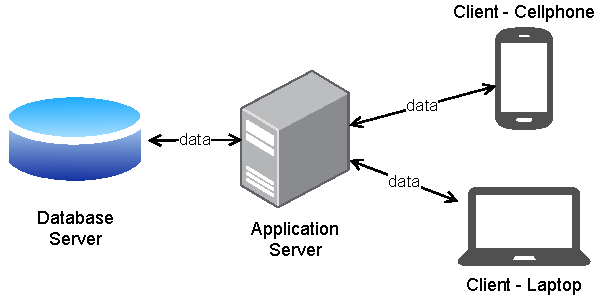
\includegraphics[width=\textwidth]{../images/client-server-3-tier}
\caption{Skema dari 3-tier client-server arsitektur.}
\label{fig:client-server-schema}
\end{figure}

\subsection{Kelebihan dan Kekurangan}
Berikut adalah kelebihan dan kekurangan arsitektur client-server:

\subsubsection{Kelebihan}
Keuntungan dari menerapkan arsitektur client-server adalah:
\begin{itemize}
\item Kemampuan komputasi (dan penyimpanan data) dapat diakses dari berbagai lokasi berjauhan dan oleh banyak komputer/pengguna.
\item Komputasi-komputasi yang membutuhkan kinerja tinggi dapat didelegasikan ke server.
\item Data dapat disentralisasikan sehingga meningkatkan konsistensi data dan mengurangi duplikasi data.
\item  Sistem dapat menerapkan \textit{horizontal scaling }untuk skalabilitas. Horizontal scaling adalah meningkatkan kinerja komputer dengan penambahan komputer agar beban komputasi dibagi ke komputer-komputer yang tersedia. Misalnya, awalnya terdapat 10 000 requests perhari yang ditangani oleh suatu \textit{application server}. Jika \textit{application server} ditambah, maka beban tersebut dibagi di antara kedua \textit{server} tersebut. Vertical scaling adalah meningkat kinerja suatu komputer dengan menaikkan spefikasi komputer tersebut, misalnya dengan menggunakan prosesor yang lebih cepat atau meningkatkan kapasitas memori.
\end{itemize}

\subsubsection{Kekurangan}
Konsekuensi dari penerapan arsitektur client-server adalah sistem jadi lebih kompleks untuk dikelola:
\begin{itemize}
\item Biaya akan meningkat karena terdapat komponen/mesin tambahan yang perlu dikelola.
\item Faktor keamanan juga perlu diperhatikan karena server dan client beroperasi dalam suatu jaringan komputer yang mana rawan terhadap \textit{cyber attack}.
\item Perlunya koordinasi antar-komputer, misalnya komunikasi sinkron dan asinkron serta komputasi parallel.
\item Kompatibilitas antara \textit{server} dan \textit{client} maupun sesama klien.
\item Masalah-masalah yang umum terdapat pada jaringan komputer etwork problems, misalnya \textit{network latency}, kesalahan dalam konfigurasi jaringan, dsb.
\end{itemize}

\section{Contoh Kasus}

\subsection{Deskripsi}
Proyek \textbf{Currency Server} adalah aplikasi berbasis Spring Boot yang berfungsi sebagai layanan backend untuk konversi mata uang. Aplikasi ini menyediakan API REST yang memungkinkan pengguna menambahkan nilai tukar antar mata uang dan melakukan konversi berdasarkan data yang tersedia dalam basis data. Sistem ini menggunakan Spring Data JPA untuk mengelola data dengan MySQL sebagai sistem manajemen basis data. Nilai tukar disimpan dalam entitas yang memiliki kunci komposit, sehingga setiap pasangan mata uang unik dapat dicatat secara akurat. 

Proyek \textbf{Currency Desktop} adalah aplikasi berbasis Java Swing yang berfungsi sebagai antarmuka pengguna untuk layanan konversi mata uang. Aplikasi ini memungkinkan pengguna memilih mata uang asal dan tujuan, memasukkan jumlah yang akan dikonversi, dan mendapatkan hasil konversi melalui integrasi dengan \textbf{Currency Server}. Permintaan data dikirimkan menggunakan koneksi HTTP, dan hasil yang dikembalikan dalam format JSON diproses menggunakan pustaka \textit{Jackson}. Dengan desain berbasis GUI, aplikasi ini memberikan pengalaman pengguna yang lebih interaktif dibandingkan dengan penggunaan API secara langsung.

Kedua proyek ini dirancang untuk bekerja secara terintegrasi, di mana \textbf{Currency Desktop} bertindak sebagai klien yang berkomunikasi dengan \textbf{Currency Server} melalui permintaan HTTP. Dengan arsitektur berbasis layanan ini, sistem dapat dikembangkan lebih lanjut untuk mendukung lebih banyak mata uang, memperluas cakupan API, atau bahkan mengintegrasikan data dari sumber eksternal lainnya.

\subsection{Server}

\subsubsection{Prasyarat}
Sebelum mengatur proyek Maven, pastikan perangkat lunak berikut telah terinstal di sistem Anda:

\begin{itemize}
\item \textbf{Java Development Kit (JDK) 11} (atau versi yang kompatibel)
\item \textbf{Apache Maven} (versi terbaru direkomendasikan)
\item \textbf{MySQL Server} (jika ingin menguji konektivitas database secara lokal)
\item \textbf{Spring Boot Dependencies}
\item \textbf{Koneksi Internet} (untuk mengunduh dependensi yang diperlukan dari repositori Maven)
\end{itemize}

\subsubsection{Instalasi Java dan Maven}
Untuk menginstal Java Development Kit (JDK) dan Maven, ikuti langkah-langkah berikut:

\begin{itemize}
\item \textbf{Instalasi Java (JDK 11)}
\begin{lstlisting}[language=bash]
sudo apt update
sudo apt install openjdk-11-jdk
java -version
\end{lstlisting}
Perintah terakhir akan menampilkan versi Java yang terinstal.

\item \textbf{Instalasi Maven}
\begin{lstlisting}[language=bash]
sudo apt update
sudo apt install maven
mvn -version
\end{lstlisting}
Perintah terakhir akan menampilkan versi Maven yang terinstal.
\end{itemize}

\subsubsection{Membuat Proyek Maven}
Untuk membuat proyek Maven baru, gunakan perintah berikut:

\begin{lstlisting}[language=bash]
mvn archetype:generate -DgroupId=pradita.softwarearchitecture -DartifactId=currency-server -DarchetypeArtifactId=maven-archetype-quickstart -DinteractiveMode=false
\end{lstlisting}

Perintah ini akan menghasilkan struktur proyek Maven dasar. Namun, konfigurasi default perlu dimodifikasi agar sesuai dengan `pom.xml` yang diberikan.

\subsubsection{Mengganti `pom.xml` Default}
Gantilah `pom.xml` yang dihasilkan dengan konten yang telah disediakan. `pom.xml` yang diberikan mencakup:

\begin{itemize}
\item \textbf{Spring Boot dependencies} (`spring-boot-starter-web`, `spring-boot-starter-data-jpa`)
\item \textbf{JUnit untuk pengujian}
\item \textbf{MySQL JDBC Connector} untuk konektivitas database
\item \textbf{Plugin Management untuk siklus hidup build Maven}
\end{itemize}

\subsubsection{Memahami Konfigurasi `pom.xml`}

\begin{itemize}
\item \textbf{Parent POM:}
\begin{lstlisting}[language=xml]
<parent>
<groupId>org.springframework.boot</groupId>
<artifactId>spring-boot-starter-parent</artifactId>
<version>2.7.8</version>
</parent>
\end{lstlisting}
Parent ini mewarisi konfigurasi dari `spring-boot-starter-parent`, yang menyederhanakan manajemen dependensi dan menyediakan konfigurasi default untuk plugin.

\item \textbf{Dependensi:}
\begin{itemize}
\item \textbf{JUnit (`test` scope)} untuk pengujian unit
\item \textbf{Spring Boot Web Starter} (`spring-boot-starter-web`) untuk membuat REST API
\item \textbf{Spring Boot JPA Starter} (`spring-boot-starter-data-jpa`) untuk interaksi database
\item \textbf{MySQL Connector} (`mysql-connector-java`) untuk konektivitas database MySQL
\end{itemize}

\item \textbf{Build Plugins:}
Bagian `<pluginManagement>` mendefinisikan plugin build Maven yang diperlukan untuk memastikan versi yang konsisten. Ini mencakup:
\begin{itemize}
\item \textbf{`maven-compiler-plugin`} (untuk mengatur versi Java ke 11)
\item \textbf{`maven-surefire-plugin`} (untuk menjalankan pengujian unit)
\item \textbf{`maven-jar-plugin`} (untuk mengemas proyek sebagai file JAR)
\item \textbf{`maven-deploy-plugin`} (untuk mendistribusikan artefak)
\end{itemize}
\end{itemize}

\subsubsection{Menambahkan Konfigurasi Tambahan}
Selain `pom.xml`, proyek memerlukan konfigurasi tambahan:

\begin{itemize}
\item \textbf{`application.properties` (Konfigurasi Spring Boot):}
Buat file `src/main/resources/application.properties` dan tambahkan konfigurasi berikut:

\begin{lstlisting}[language=ini]
spring.jpa.hibernate.ddl-auto=create-drop
spring.datasource.url=jdbc:mysql://localhost:3306/currency
spring.datasource.username=alfa
spring.datasource.password=1234
spring.datasource.driver-class-name=com.mysql.cj.jdbc.Driver
spring.jpa.show-sql=true
spring.jpa.defer-datasource-initialization=true
spring.sql.init.mode=always
\end{lstlisting}

Konfigurasi ini memastikan bahwa database `currency` dibuat ulang setiap kali aplikasi dijalankan, menggunakan MySQL sebagai database utama dengan kredensial yang telah disesuaikan.
\end{itemize}


\subsubsection{Membangun dan Menjalankan Proyek}
Setelah struktur proyek dikonfigurasi, jalankan perintah berikut:

\begin{itemize}
\item \textbf{Untuk membangun proyek:}
\begin{lstlisting}[language=bash]
mvn clean package
\end{lstlisting}

\item \textbf{Untuk menjalankan proyek:}
\begin{lstlisting}[language=bash]
mvn spring-boot:run
\end{lstlisting}

Perintah ini akan memulai aplikasi Spring Boot dan mengekspos API yang telah didefinisikan dalam proyek.
\end{itemize}

\subsubsection{Memverifikasi Setup}
Setelah aplikasi berjalan, verifikasi dengan mengakses:

\begin{lstlisting}
http://localhost:8080/
\end{lstlisting}

Jika semuanya telah dikonfigurasi dengan benar, aplikasi Spring Boot akan berjalan dengan sukses.


\subsubsection{Membuat File \texttt{RateId.java}}
Buatlah file `RateId.java` di dalam direktori `src/main/java/pradita/softwarearchitecture/chapter02/`. File ini akan digunakan sebagai kunci utama dalam entitas JPA yang memetakan pasangan mata uang.

Ikuti langkah-langkah berikut untuk membuat file `RateId.java`:

\begin{enumerate}
\item Navigasikan ke direktori proyek Anda menggunakan terminal atau file explorer.
\item Buat folder `chapter02` jika belum ada dengan perintah berikut di terminal:

\begin{lstlisting}[language=bash]
mkdir -p src/main/java/pradita/softwarearchitecture/chapter02
\end{lstlisting}

\item Buat file baru dengan nama `RateId.java` menggunakan perintah:

\begin{lstlisting}[language=bash]
touch src/main/java/pradita/softwarearchitecture/chapter02/RateId.java
\end{lstlisting}

\item Buka file tersebut dengan editor pilihan Anda dan salin kode berikut:

\begin{lstlisting}[style=JavaStyle]
package pradita.softwarearchitecture.chapter02;

import java.io.Serializable;

public class RateId implements Serializable {
	private String fromCurrency;
	private String toCurrency;
	
	public String getFromCurrency() {
		return this.fromCurrency;
	}
	
	public void setFromCurrency(String fromCurrency) {
		this.fromCurrency = fromCurrency;
	}
	
	public String getToCurrency() {
		return this.toCurrency;
	}
	
	public void setToCurrency(String toCurrency) {
		this.toCurrency = toCurrency;
	}
}
\end{lstlisting}

\item Simpan perubahan dan pastikan file sudah tersimpan dalam lokasi yang benar.
\end{enumerate}

Setelah file `RateId.java` dibuat, Anda dapat menggunakannya dalam entitas JPA dengan anotasi `@IdClass` atau `@Embeddable` untuk mengelola kunci komposit dalam basis data.


\subsubsection{Membuat File \texttt{RateRepository.java}}
File `RateRepository.java` perlu dibuat di dalam direktori `src/main/java/pradita/softwarearchitecture/chapter02/`. File ini berfungsi sebagai \textit{repository} dalam Spring Data JPA yang memungkinkan operasi CRUD terhadap entitas `Rate`.

Spring Data JPA menyediakan antarmuka `CrudRepository` yang secara otomatis menangani operasi database tanpa memerlukan implementasi manual. Pada kelas ini, metode \texttt{findFirstByFromCurrencyAndToCurrency} digunakan untuk melakukan pencarian data berdasarkan pasangan mata uang yang diberikan.

\textbf{Langkah-langkah Membuat File \texttt{RateRepository.java}:}

\begin{enumerate}
\item Buka terminal atau file explorer dan navigasikan ke direktori proyek.
\item Jika folder `chapter02` belum ada, buat dengan perintah berikut:

\begin{lstlisting}[language=bash]
mkdir -p src/main/java/pradita/softwarearchitecture/chapter02
\end{lstlisting}

\item Buat file baru dengan nama `RateRepository.java` menggunakan perintah:

\begin{lstlisting}[language=bash]
touch src/main/java/pradita/softwarearchitecture/chapter02/RateRepository.java
\end{lstlisting}

\item Buka file dengan editor pilihan dan masukkan kode berikut:

\begin{lstlisting}[style=JavaStyle]
package pradita.softwarearchitecture.chapter02;

import java.util.Collection;
import org.springframework.data.repository.CrudRepository;

public interface RateRepository extends CrudRepository<Rate, Integer> {
	
	// JPQL Query (dikomentari untuk referensi)
	//@Query("SELECT r FROM Rate r WHERE r.fromCurrency = ?1 and r.toCurrency = ?2")
	
	// Metode ini mencari data berdasarkan pasangan mata uang fromCurrency dan toCurrency.
	Collection<Rate> findFirstByFromCurrencyAndToCurrency(String fromCurrency, String toCurrency);
}
\end{lstlisting}

\item Simpan perubahan dan pastikan file tersimpan dalam lokasi yang benar.
\end{enumerate}

\subsubsection{Penjelasan Kode}
\begin{itemize}
\item \textbf{Paket:} Kelas ini berada dalam paket `pradita.softwarearchitecture.chapter02`, yang menunjukkan bahwa ini merupakan bagian dari struktur proyek.
\item \textbf{Antarmuka \texttt{CrudRepository}:} 
\begin{itemize}
\item `RateRepository` memperluas `CrudRepository<Rate, Integer>`, yang menyediakan operasi dasar seperti `save`, `findById`, `findAll`, dan `delete` tanpa implementasi manual.
\item `Rate` adalah entitas yang dikelola, sedangkan `Integer` adalah tipe data dari kunci utama entitas `Rate`.
\end{itemize}
\item \textbf{Metode Kustom:}
\begin{itemize}
\item \texttt{findFirstByFromCurrencyAndToCurrency}:  
\begin{itemize}
	\item Metode ini secara otomatis diterjemahkan oleh Spring Data JPA menjadi kueri database yang mencari \textbf{data pertama} berdasarkan mata uang asal (`fromCurrency`) dan mata uang tujuan (`toCurrency`).
	\item Jika metode ini digunakan tanpa anotasi `@Query`, Spring Data JPA akan menerjemahkannya ke dalam sintaks SQL atau JPQL secara otomatis.
\end{itemize}
\end{itemize}
\end{itemize}

Setelah file `RateRepository.java` dibuat, penggunaannya dalam layanan Spring Boot memungkinkan pengambilan data berdasarkan pasangan mata uang dengan efisiensi tinggi menggunakan fitur bawaan dari Spring Data JPA.


\subsubsection{Membuat File \texttt{Rate.java}}
File `Rate.java` perlu dibuat di dalam direktori `src/main/java/pradita/softwarearchitecture/chapter02/`. File ini berfungsi sebagai entitas dalam JPA yang merepresentasikan data nilai tukar mata uang dengan menggunakan kunci komposit.

Spring Data JPA menyediakan anotasi `@Entity` untuk menandai kelas ini sebagai entitas yang akan dipetakan ke dalam tabel database. Anotasi `@IdClass(RateId.class)` digunakan untuk menentukan bahwa entitas ini memiliki kunci komposit yang terdiri dari dua atribut: `fromCurrency` dan `toCurrency`.

\textbf{Langkah-langkah Membuat File \texttt{Rate.java}:}

\begin{enumerate}
\item Buka terminal atau file explorer dan navigasikan ke direktori proyek.
\item Jika folder `chapter02` belum ada, buat dengan perintah berikut:

\begin{lstlisting}[language=bash]
mkdir -p src/main/java/pradita/softwarearchitecture/chapter02
\end{lstlisting}

\item Buat file baru dengan nama `Rate.java` menggunakan perintah:

\begin{lstlisting}[language=bash]
touch src/main/java/pradita/softwarearchitecture/chapter02/Rate.java
\end{lstlisting}

\item Buka file dengan editor pilihan dan masukkan kode berikut:

\begin{lstlisting}[style=JavaStyle]
package pradita.softwarearchitecture.chapter02;

import javax.persistence.Entity;
import javax.persistence.Id;
import javax.persistence.IdClass;

@Entity
@IdClass(RateId.class)
public class Rate {
	
	@Id
	private String fromCurrency;
	@Id
	private String toCurrency;
	private Double rate;
	
	Rate(){
		super();
	}
	
	Rate(String fromCurrency, String toCurrency, Double rate) {
		super();
		this.fromCurrency = fromCurrency;
		this.toCurrency = toCurrency;
		this.rate = rate;
	}
	
	public String getFromCurrency() {
		return this.fromCurrency;
	}
	
	public void setFromCurrency(String fromCurrency) {
		this.fromCurrency = fromCurrency;
	}
	
	public String getToCurrency() {
		return this.toCurrency;
	}
	
	public void setToCurrency(String toCurrency) {
		this.toCurrency = toCurrency;
	}
	
	public Double getRate() {
		return this.rate;
	}
	
	public void setRate(Double rate) {
		this.rate = rate;
	}
}
\end{lstlisting}

\item Simpan perubahan dan pastikan file tersimpan dalam lokasi yang benar.
\end{enumerate}

\subsubsection{Penjelasan Kode}
\begin{itemize}
\item \textbf{Paket:} Kelas ini berada dalam paket `pradita.softwarearchitecture.chapter02`, yang menunjukkan bahwa ini merupakan bagian dari struktur proyek.
\item \textbf{Anotasi JPA:}
\begin{itemize}
\item `@Entity` digunakan untuk menandai kelas ini sebagai entitas yang akan dipetakan ke tabel dalam database.
\item `@IdClass(RateId.class)` menunjukkan bahwa kelas ini menggunakan kunci komposit yang didefinisikan dalam kelas `RateId`.
\item `@Id` diberikan pada atribut `fromCurrency` dan `toCurrency`, yang berarti kedua atribut ini membentuk kunci utama entitas `Rate`.
\end{itemize}
\item \textbf{Atribut:}
\begin{itemize}
\item `fromCurrency` - Mewakili mata uang asal dalam pasangan nilai tukar.
\item `toCurrency` - Mewakili mata uang tujuan dalam pasangan nilai tukar.
\item `rate` - Menyimpan nilai tukar antara dua mata uang yang diberikan.
\end{itemize}
\item \textbf{Konstruktor:}
\begin{itemize}
\item Konstruktor tanpa parameter (`Rate()`) diperlukan oleh JPA agar dapat membuat instance objek secara otomatis.
\item Konstruktor dengan parameter digunakan untuk menginisialisasi objek `Rate` dengan nilai `fromCurrency`, `toCurrency`, dan `rate`.
\end{itemize}
\item \textbf{Metode Getter dan Setter:}
\begin{itemize}
\item Metode `getFromCurrency()` dan `setFromCurrency()` digunakan untuk mendapatkan dan mengubah nilai mata uang asal.
\item Metode `getToCurrency()` dan `setToCurrency()` digunakan untuk mendapatkan dan mengubah nilai mata uang tujuan.
\item Metode `getRate()` dan `setRate()` digunakan untuk mendapatkan dan mengubah nilai tukar.
\end{itemize}
\end{itemize}

Setelah file `Rate.java` dibuat, kelas ini dapat digunakan dalam kombinasi dengan repository JPA untuk menyimpan dan mengambil data nilai tukar mata uang dalam basis data secara otomatis.

\subsubsection{Membuat File \texttt{App.java}}
File `App.java` perlu dibuat di dalam direktori `src/main/java/pradita/softwarearchitecture/chapter02/`. File ini berfungsi sebagai kelas utama dalam aplikasi Spring Boot yang menyediakan endpoint REST untuk menambahkan dan mengonversi nilai tukar mata uang.

Spring Boot menyediakan anotasi `@SpringBootApplication` untuk mengonfigurasi aplikasi secara otomatis, sementara anotasi `@RestController` memungkinkan kelas ini menangani permintaan HTTP dan memberikan respons dalam format JSON.

\textbf{Langkah-langkah Membuat File \texttt{App.java}:}

\begin{enumerate}
\item Buka terminal atau file explorer dan navigasikan ke direktori proyek.
\item Jika folder `chapter02` belum ada, buat dengan perintah berikut:

\begin{lstlisting}[language=bash]
mkdir -p src/main/java/pradita/softwarearchitecture/chapter02
\end{lstlisting}

\item Buat file baru dengan nama `App.java` menggunakan perintah:

\begin{lstlisting}[language=bash]
touch src/main/java/pradita/softwarearchitecture/chapter02/App.java
\end{lstlisting}

\item Buka file dengan editor pilihan dan masukkan kode berikut:

\begin{lstlisting}[style=JavaStyle]
package pradita.softwarearchitecture.chapter02;

import java.util.Collection;
import java.util.HashMap;
import java.util.Map;

import org.springframework.beans.factory.annotation.Autowired;
import org.springframework.boot.SpringApplication;
import org.springframework.boot.autoconfigure.SpringBootApplication;
import org.springframework.http.MediaType;
import org.springframework.web.bind.annotation.RequestMapping;
import org.springframework.web.bind.annotation.RestController;

@RestController
@SpringBootApplication
public class App {
	
	@Autowired
	private RateRepository rateRepository;
	
	public static void main(String[] args) {
		SpringApplication.run(App.class, args);
	}
	
	@RequestMapping("/")
	String home() {
		return "Hello World!";
	}
	
	@RequestMapping(path = "/addrate", produces = MediaType.APPLICATION_JSON_VALUE)
	Rate addRate(String from, String to, Double rate) {
		Rate r = new Rate(from, to, rate);
		rateRepository.save(r);
		return r;
	}
	
	@RequestMapping(path = "/convert", produces = MediaType.APPLICATION_JSON_VALUE)
	Map<String, Object> convert(Double value, String from, String to) {
		Map<String, Object> result = new HashMap<>();
		result.put("fromCurrency", from);
		result.put("toCurrency", to);
		Double rate = 0d;
		Collection<Rate> rates = rateRepository.findFirstByFromCurrencyAndToCurrency(from, to);
		if (rates.size() > 0) {
			Rate r = rates.iterator().next();
			rate = r.getRate();
		}
		result.put("rate", rate);
		result.put("value", rate * value);
		return result;
	}
}
\end{lstlisting}

\item Simpan perubahan dan pastikan file tersimpan dalam lokasi yang benar.
\end{enumerate}

\subsubsection{Penjelasan Kode}
\begin{itemize}
\item \textbf{Paket:} Kelas ini berada dalam paket `pradita.softwarearchitecture.chapter02`, yang menunjukkan bahwa ini merupakan bagian dari struktur proyek.
\item \textbf{Anotasi Spring Boot:}
\begin{itemize}
\item `@SpringBootApplication` digunakan untuk mengonfigurasi aplikasi Spring Boot secara otomatis.
\item `@RestController` memungkinkan kelas ini menangani permintaan HTTP dan memberikan respons dalam format JSON.
\end{itemize}
\item \textbf{Atribut:}
\begin{itemize}
\item `rateRepository` adalah objek `RateRepository` yang digunakan untuk mengakses data nilai tukar mata uang dalam basis data.
\end{itemize}
\item \textbf{Metode:}
\begin{itemize}
\item \texttt{main(String[] args)}: 
\begin{itemize}
	\item Metode utama yang menjalankan aplikasi Spring Boot dengan `SpringApplication.run(App.class, args)`.
\end{itemize}
\item \texttt{home()}: 
\begin{itemize}
	\item Endpoint `"/"` yang mengembalikan teks `"Hello World!"` ketika diakses.
\end{itemize}
\item \texttt{addRate(String from, String to, Double rate)}:
\begin{itemize}
	\item Menyediakan endpoint `"/addrate"` untuk menambahkan nilai tukar mata uang baru ke dalam database.
	\item Parameter `from`, `to`, dan `rate` dikonversi menjadi objek `Rate` yang kemudian disimpan ke dalam database melalui `rateRepository.save(r)`.
\end{itemize}
\item \texttt{convert(Double value, String from, String to)}:
\begin{itemize}
	\item Menyediakan endpoint `"/convert"` untuk mengonversi mata uang berdasarkan nilai tukar yang tersimpan di database.
	\item Melakukan pencarian nilai tukar dengan metode `findFirstByFromCurrencyAndToCurrency(from, to)`.
	\item Jika nilai tukar ditemukan, hasil konversi dihitung dan dikembalikan dalam bentuk JSON.
\end{itemize}
\end{itemize}
\end{itemize}

Setelah file `App.java` dibuat, kelas ini akan menjadi titik masuk utama untuk menjalankan aplikasi Spring Boot serta menyediakan layanan REST API untuk menambahkan dan mengonversi nilai tukar mata uang.

\subsection{Dekstop Client}

\subsubsection{Menyiapkan Proyek Maven untuk \texttt{currency-desktop}}
Proyek \texttt{currency-desktop} merupakan aplikasi berbasis Java yang menggunakan Maven sebagai manajer proyek dan pustaka. Konfigurasi yang diberikan dalam berkas `pom.xml` menentukan dependensi yang dibutuhkan serta pengaturan kompilasi proyek.

\textbf{Langkah-langkah Menyiapkan Proyek:}

\begin{enumerate}
\item Buka terminal atau file explorer dan navigasikan ke direktori tempat proyek akan dibuat.
\item Gunakan perintah berikut untuk membuat proyek Maven baru:

\begin{lstlisting}[language=bash]
mvn archetype:generate -DgroupId=pradita.softwarearchitecture -DartifactId=currency-desktop -DarchetypeArtifactId=maven-archetype-quickstart -DinteractiveMode=false
\end{lstlisting}

\item Gantilah berkas `pom.xml` yang dihasilkan dengan konfigurasi berikut:

\begin{lstlisting}[language=xml]
<?xml version="1.0" encoding="UTF-8"?>

<project xmlns="http://maven.apache.org/POM/4.0.0"
xmlns:xsi="http://www.w3.org/2001/XMLSchema-instance" xsi:schemaLocation="http://maven.apache.org/POM/4.0.0 http://maven.apache.org/xsd/maven-4.0.0.xsd">
<modelVersion>4.0.0</modelVersion>

<groupId>pradita.softwarearchitecture</groupId>
<artifactId>currency-desktop</artifactId>
<version>1.0-SNAPSHOT</version>

<name>currency-desktop</name>
<url>http://www.example.com</url>

<properties>
<project.build.sourceEncoding>UTF-8</project.build.sourceEncoding>
<maven.compiler.source>11</maven.compiler.source>
<maven.compiler.target>11</maven.compiler.target>
</properties>

<dependencies>
<dependency>
<groupId>junit</groupId>
<artifactId>junit</artifactId>
<version>4.11</version>
<scope>test</scope>
</dependency>
<dependency>
<groupId>com.fasterxml.jackson.core</groupId>
<artifactId>jackson-core</artifactId>
<version>2.14.2</version>
</dependency>
<dependency>
<groupId>com.fasterxml.jackson.core</groupId>
<artifactId>jackson-databind</artifactId>
<version>2.14.2</version>
</dependency>
</dependencies>

<build>
<pluginManagement>
<plugins>
<plugin>
<artifactId>maven-clean-plugin</artifactId>
<version>3.1.0</version>
</plugin>
<plugin>
<artifactId>maven-resources-plugin</artifactId>
<version>3.0.2</version>
</plugin>
<plugin>
<artifactId>maven-compiler-plugin</artifactId>
<version>3.8.0</version>
</plugin>
<plugin>
<artifactId>maven-surefire-plugin</artifactId>
<version>2.22.1</version>
</plugin>
<plugin>
<artifactId>maven-jar-plugin</artifactId>
<version>3.0.2</version>
</plugin>
<plugin>
<artifactId>maven-install-plugin</artifactId>
<version>2.5.2</version>
</plugin>
<plugin>
<artifactId>maven-deploy-plugin</artifactId>
<version>2.8.2</version>
</plugin>
<plugin>
<artifactId>maven-site-plugin</artifactId>
<version>3.7.1</version>
</plugin>
<plugin>
<artifactId>maven-project-info-reports-plugin</artifactId>
<version>3.0.0</version>
</plugin>
</plugins>
</pluginManagement>
</build>
</project>
\end{lstlisting}

\item Simpan perubahan dan pastikan `pom.xml` sudah dikonfigurasi dengan benar.
\end{enumerate}

\subsubsection{Penjelasan Konfigurasi}
\begin{itemize}
\item \textbf{Grup dan Artefak:}  
\begin{itemize}
\item `groupId`: \texttt{pradita.softwarearchitecture} - Menentukan nama grup proyek.
\item `artifactId`: \texttt{currency-desktop} - Menentukan nama proyek.
\item `version`: `1.0-SNAPSHOT` - Menentukan versi proyek.
\end{itemize}
\item \textbf{Properti Maven:}
\begin{itemize}
\item `maven.compiler.source` dan `maven.compiler.target` diatur ke `11`, menunjukkan bahwa proyek dikompilasi menggunakan Java 11.
\end{itemize}
\item \textbf{Dependensi:}
\begin{itemize}
\item `junit` - Digunakan untuk menjalankan pengujian unit.
\item `jackson-core` - Pustaka untuk memproses JSON dalam Java.
\item `jackson-databind` - Pustaka untuk serialisasi dan deserialisasi objek Java ke JSON.
\end{itemize}
\item \textbf{Pengelolaan Plugin:}
\begin{itemize}
\item `maven-clean-plugin` - Membersihkan artefak build sebelum memulai proses baru.
\item `maven-compiler-plugin` - Mengompilasi kode sumber proyek.
\item `maven-jar-plugin` - Menghasilkan file \texttt{.jar} dari proyek.
\item `maven-surefire-plugin` - Menjalankan pengujian unit secara otomatis.
\item `maven-install-plugin` - Menginstal artefak ke lokal repository.
\item `maven-deploy-plugin` - Mengunggah artefak ke repository eksternal.
\item `maven-site-plugin` - Menghasilkan dokumentasi proyek berbasis situs.
\item `maven-project-info-reports-plugin` - Menyediakan laporan informasi proyek.
\end{itemize}
\end{itemize}

\subsubsection{Membangun dan Menjalankan Proyek}
Setelah konfigurasi selesai, gunakan perintah berikut untuk membangun dan menjalankan proyek:

\begin{itemize}
\item Untuk membersihkan proyek:
\begin{lstlisting}[language=bash]
mvn clean
\end{lstlisting}

\item Untuk membangun proyek:
\begin{lstlisting}[language=bash]
mvn package
\end{lstlisting}

\item Untuk menjalankan aplikasi:
\begin{lstlisting}[language=bash]
java -jar target/currency-desktop-1.0-SNAPSHOT.jar
\end{lstlisting}
\end{itemize}

Dengan mengikuti langkah-langkah di atas, proyek \texttt{currency-desktop} akan siap untuk dijalankan menggunakan Maven dan Java 11.

\subsubsection{Membuat File \texttt{CurrencyDesktop.java}}
File `CurrencyDesktop.java` perlu dibuat di dalam direktori `src/main/java/pradita/softwarearchitecture/chapter02/`. File ini berfungsi sebagai aplikasi GUI berbasis Swing yang memungkinkan pengguna mengonversi nilai mata uang dengan menghubungkan ke layanan backend.

Aplikasi ini menggunakan `JFrame` dan komponen Swing lainnya untuk membangun antarmuka pengguna yang interaktif. Proses konversi dilakukan dengan mengirimkan permintaan HTTP ke server yang menjalankan layanan konversi mata uang.

\textbf{Langkah-langkah Membuat File \texttt{CurrencyDesktop.java}:}

\begin{enumerate}
\item Buka terminal atau file explorer dan navigasikan ke direktori proyek.
\item Jika folder `chapter02` belum ada, buat dengan perintah berikut:

\begin{lstlisting}[language=bash]
mkdir -p src/main/java/pradita/softwarearchitecture/chapter02
\end{lstlisting}

\item Buat file baru dengan nama `CurrencyDesktop.java` menggunakan perintah:

\begin{lstlisting}[language=bash]
touch src/main/java/pradita/softwarearchitecture/chapter02/CurrencyDesktop.java
\end{lstlisting}

\item Buka file dengan editor pilihan dan masukkan kode berikut:

\begin{lstlisting}[style=JavaStyle]
package pradita.softwarearchitecture.chapter02;

import java.awt.Point;
import java.awt.GraphicsEnvironment;
import java.awt.EventQueue;
import java.awt.Font;
import java.awt.event.ActionEvent;
import java.awt.event.ActionListener;
import java.io.BufferedReader;
import java.io.IOException;
import java.io.InputStream;
import java.io.InputStreamReader;
import java.io.UnsupportedEncodingException;
import java.net.HttpURLConnection;
import java.net.URL;
import java.net.URLEncoder;
import java.util.HashMap;
import java.util.Map;

import javax.swing.*;

import com.fasterxml.jackson.databind.JsonNode;
import com.fasterxml.jackson.databind.ObjectMapper;

public class CurrencyDesktop extends JFrame {
	
	private static final long serialVersionUID = 1L;
	private JPanel contentPane;
	private JTextField textFieldValue;
	
	public static void main(String[] args) {
		EventQueue.invokeLater(new Runnable() {
			public void run() {
				try {
					CurrencyDesktop frame = new CurrencyDesktop();
					frame.setVisible(true);
				} catch (Exception e) {
					e.printStackTrace();
				}
			}
		});
	}
	
	public CurrencyDesktop() {
		setTitle("Currency Converter");
		setDefaultCloseOperation(JFrame.EXIT_ON_CLOSE);
		setBounds(100, 100, 493, 130);
		contentPane = new JPanel();
		contentPane.setBorder(new EmptyBorder(5, 5, 5, 5));
		setContentPane(contentPane);
		contentPane.setLayout(null);
		
		Point centerPoint = GraphicsEnvironment.getLocalGraphicsEnvironment().getCenterPoint();
		this.setLocation(centerPoint.x - (int) this.getSize().getWidth() / 2,
		centerPoint.y - (int) this.getSize().getHeight() / 2);
		
		JLabel labelFrom = new JLabel("From");
		labelFrom.setFont(new Font("SansSerif", Font.PLAIN, 20));
		labelFrom.setBounds(16, 20, 63, 16);
		contentPane.add(labelFrom);
		
		JComboBox<String> comboBoxFrom = new JComboBox<>(new String[] { "USD", "GBP", "JPY" });
		comboBoxFrom.setFont(new Font("SansSerif", Font.PLAIN, 20));
		comboBoxFrom.setBounds(81, 15, 111, 26);
		contentPane.add(comboBoxFrom);
		
		JLabel labelTo = new JLabel("To");
		labelTo.setFont(new Font("SansSerif", Font.PLAIN, 20));
		labelTo.setBounds(16, 53, 63, 16);
		contentPane.add(labelTo);
		
		JComboBox<String> comboBoxTo = new JComboBox<>(new String[] { "IDR", "GBP" });
		comboBoxTo.setFont(new Font("SansSerif", Font.PLAIN, 20));
		comboBoxTo.setBounds(81, 48, 111, 26);
		contentPane.add(comboBoxTo);
		
		textFieldValue = new JTextField("1.0");
		textFieldValue.setHorizontalAlignment(SwingConstants.RIGHT);
		textFieldValue.setFont(new Font("SansSerif", Font.PLAIN, 20));
		textFieldValue.setBounds(204, 14, 112, 28);
		contentPane.add(textFieldValue);
		
		JLabel lblConvertedValue = new JLabel("");
		lblConvertedValue.setFont(new Font("SansSerif", Font.PLAIN, 20));
		lblConvertedValue.setHorizontalAlignment(SwingConstants.RIGHT);
		lblConvertedValue.setBounds(204, 48, 112, 26);
		contentPane.add(lblConvertedValue);
		
		JButton btnConvert = new JButton("Convert");
		btnConvert.setFont(new Font("SansSerif", Font.PLAIN, 20));
		btnConvert.setBounds(322, 14, 132, 27);
		contentPane.add(btnConvert);
		
		btnConvert.addActionListener(new ActionListener() {
			public void actionPerformed(ActionEvent e) {
				try {
					Map<String, String> params = new HashMap<>();
					params.put("from", comboBoxFrom.getSelectedItem().toString());
					params.put("to", comboBoxTo.getSelectedItem().toString());
					params.put("value", textFieldValue.getText());
					String paramString = getParamsString(params);
					String getUrl = "http://localhost:8080/convert?" + paramString;
					double convertedValue = getAmount(getUrl);
					lblConvertedValue.setText(String.valueOf(convertedValue));
				} catch (Exception exception) {
					exception.printStackTrace();
				}
			}
		});
	}
	
	private ObjectMapper mapper = new ObjectMapper();
	
	public double getAmount(String getUrl) throws IOException {
		URL obj = new URL(getUrl);
		HttpURLConnection con = (HttpURLConnection) obj.openConnection();
		con.setRequestProperty("accept", "application/json");
		InputStream inputStream = con.getInputStream();
		BufferedReader in = new BufferedReader(new InputStreamReader(inputStream));
		String inputLine;
		StringBuffer response = new StringBuffer();
		while ((inputLine = in.readLine()) != null) {
			response.append(inputLine);
		}
		in.close();
		con.disconnect();
		
		JsonNode node = mapper.readTree(response.toString());
		return node.get("value").asDouble();
	}
	
	public static String getParamsString(Map<String, String> params) throws UnsupportedEncodingException {
		StringBuilder result = new StringBuilder();
		for (Map.Entry<String, String> entry : params.entrySet()) {
			result.append(URLEncoder.encode(entry.getKey(), "UTF-8"));
			result.append("=");
			result.append(URLEncoder.encode(entry.getValue(), "UTF-8"));
			result.append("&");
		}
		return result.toString();
	}
}
\end{lstlisting}

\item Simpan perubahan dan pastikan file tersimpan dalam lokasi yang benar.
\end{enumerate}

\subsubsection{Penjelasan Kode}
\begin{itemize}
\item \textbf{Paket:} Kelas ini berada dalam paket `pradita.softwarearchitecture.chapter02`.
\item \textbf{Antarmuka Pengguna:}
\begin{itemize}
\item Menggunakan `JFrame` dan komponen Swing seperti `JComboBox`, `JButton`, dan `JLabel` untuk antarmuka pengguna.
\end{itemize}
\item \textbf{Fungsi Konversi:}
\begin{itemize}
\item Menggunakan `HttpURLConnection` untuk mengirim permintaan HTTP ke server dan mendapatkan hasil konversi.
\item `getAmount(String getUrl)` mengambil nilai tukar dari server dan mengembalikannya sebagai `double`.
\end{itemize}
\end{itemize}

Setelah `CurrencyDesktop.java` dibuat, aplikasi ini dapat digunakan sebagai antarmuka desktop untuk mengonversi nilai mata uang.

\subsection{Kesimpulan}

Arsitektur perangkat lunak memainkan peran penting dalam pengembangan sistem yang scalable, dapat diandalkan, dan mudah dikelola. Prinsip-prinsip dan teknik yang digunakan dalam perancangan arsitektur berkontribusi terhadap efisiensi sistem serta kemampuannya dalam menangani perubahan kebutuhan bisnis dan teknologi.

Studi kasus yang telah dibahas menunjukkan dampak langsung dari keputusan arsitektur terhadap keberhasilan dan kegagalan sistem perangkat lunak. Transformasi dari arsitektur monolitik ke mikroservis, kegagalan implementasi sistem yang tidak mempertimbangkan desain arsitektural dengan baik, serta penerapan arsitektur event-driven dalam sistem perbankan adalah beberapa contoh bagaimana arsitektur perangkat lunak mempengaruhi keberlangsungan sebuah sistem.

Arsitektur \textit{Client-Server} merupakan salah satu pendekatan fundamental dalam pengembangan sistem terdistribusi. Dengan membagi peran server sebagai penyedia layanan dan klien sebagai pengguna layanan, pendekatan ini menawarkan fleksibilitas, skalabilitas, serta efisiensi dalam pengelolaan sumber daya. Meskipun memiliki kelebihan dalam pengelolaan data yang terpusat, arsitektur ini juga memiliki tantangan seperti ketersediaan dan performa server.

Sebagai studi kasus, implementasi proyek \textit{Currency Server} dan \textit{Currency Desktop} menggambarkan bagaimana arsitektur client-server diterapkan dalam sistem konversi mata uang. \textit{Currency Server} bertindak sebagai backend yang menyediakan layanan melalui API REST, sedangkan \textit{Currency Desktop} berfungsi sebagai klien yang berinteraksi dengan server untuk mendapatkan data nilai tukar. Integrasi antara kedua sistem ini menunjukkan bagaimana arsitektur client-server dapat mendukung komunikasi antara komponen yang berbeda dalam lingkungan perangkat lunak yang terdistribusi.

Dengan memahami konsep dan penerapan arsitektur perangkat lunak, pengembangan sistem dapat dilakukan dengan lebih terstruktur dan efisien. Pemilihan arsitektur yang tepat berdasarkan kebutuhan sistem akan berkontribusi terhadap keberlanjutan dan keberhasilan implementasi perangkat lunak dalam jangka panjang.
